% Template pour poster.

\documentclass{beamer}
\usepackage[T1]{fontenc}
\usepackage[utf8]{inputenc}

\usepackage{array}
\usepackage{amstext}
\usepackage{graphicx}
\makeatletter
\usepackage{multirow}
\usepackage{color}
\usepackage{exscale}
\usepackage{pifont}
\usepackage{xspace}
\usepackage{array}
\usepackage{subfigure}

% NOTE: le paramètre scale permet d'augmenter la taille des polices partout 
% dans le document
\usepackage[orientation=portrait, size=a0, scale=1.5]{beamerposter}

\usetheme{olibposter}

% Set colors for blocks (without frame)
\setbeamercolor{block title}{fg=dblue,bg=white}
\setbeamercolor{block body}{fg=black,bg=white}
\setbeamercolor{block alerted title}{fg=white,bg=dblue!70}%frame color
\setbeamercolor{block alerted body}{fg=black,bg=dblue!10}%body color
\setbeamertemplate{caption}[numbered]

% Titre, date, auteurs
\title{Integrated Software Project \\ Calendar Tool Application}
\author{Imperiali Michele, Lorent Nicolas, Vanosmael Laurent and Mormont Romain\\
{\tt mjimperiali@student.ulg.ac.be, nicolas.lorent@student.ulg.ac.be, laurent.vanosmael@student.ulg.ac.be, r.mormont@student.ulg.ac.be}}
\institute{Faculty of Applied Sciences -- University of Liège -- Belgium}
\date{Année académique 2013-2014}


\begin{document}

% Permet d'obtenir deux colonnes (ou plus)
% Si vous avez besoin d'insérer une image qui s'étalent sur deux colonnes, insérez la hors de l'environnement "columns", de préférence dans le bas de la page.
\begin{columns}[t]

% On déclare une première colonne faisant 45% de la largeur de la page. Tout ce qui est écrit après cette ligne et jusqu'au prochain \column fait partie de la colonne
\column{.45\paperwidth}

% Les blocks permettent de mettre en page et structurer votre document.
% À vous de choisir comment présenter votre document.
 ~~ 
\begin{alertblock}{Introduction}
The \textbf{Calendar Tool Application} is a web-based scheduling application. On the one hand, it allows students to manage their personal and educational agenda. On the other hand, it provides to professors and faculty staff members a global view of students' schedule and allows them to schedule courses, projects, etc, in an optimal way.
The application is available through a web interface and a mobile application.
\end{alertblock}

~~ % Permet de faire un paragraphe "vide" entre deux blocks.

\begin{block}{Title}
Block contnte :

\end{block}

~~
\begin{block}{Which part to optimize?}
It was clear for us that we had to put our focus in optimizing the operation that was performed the most often.
Obviously, the initialization is performed only once. The segmentation is done for each frame of the video, whereas, for each pixels in the background model, there is a probability to update it. Therefore, we decided to focus on the segmentation. 
\end{block}

~~ 
\begin{block}{Sequential implementation}
Without getting into the details, an optimization performed on the sequential version consists of maintaining the background model in two buffers. The first one contains the values that matched recently and the second contains the others. This allows to reduce the average complexity of the segmentation.
\end{block}

~~
\begin{block}{Vectorization}
Our vectorization is targeted to speed up the segmentation. It performs the distance check for all pixels of a model at once. Since this distance check is performed in one-go, we decided to use one buffer instead of two as in the sequential version. This parallelism is obtained thanks to the NEON C intrinsics which exposes a lot of useful operations on and between vectors. Nevertheless, we didn't find many aggregation operation and had to implement ourself an accumulation (see the \texttt{accumulate} step in the Figure \ref{fig:algo}).

\begin{figure}
	\center
	%\includegraphics[scale=1.35]{algo.png}
	\caption{Steps of the vectorized implementation}
	\label{fig:algo}
\end{figure}
\end{block}

\column{.45\paperwidth}
~~ 
\begin{block}{Results}
We have used the performances of the sequential implementation to assess our vectorization. The execution time of the segmentation and update steps are given in Figure \ref{fig:exec}. The chart highlights the quickness of the sequential version compared to our implementation. The former is actually two times faster than the latter and it even reaches an impressive framerate of 273 on one of the test video. 

\vspace{1cm}
\begin{figure}
	\center
	%\includegraphics[scale=2]{exectime.png}
	\label{fig:exec}
	\caption{Execution time of the segmentation and update steps ($\mu$s)}
\end{figure}
\vspace{1cm}

We think that the slowness of our implementation is due the combination of the following factors :

\begin{center}
\begin{minipage}{0.95\linewidth}
\textbf{(1)} The accumulate operation shown on Figure \ref{fig:algo} is quite expensive (it compiles in 10 assembly instructions). \\
\textbf{(2)} Our implementation uses every pixel of a model at each iteration (in the segmentation loop) while the sequential one first checks two pixels and only tests the others if necessary. \\
\textbf{(3)} On the test sequences, most of the pixels were in the background. 
\end{minipage}
\end{center}

\end{block}
~~ 
\begin{block}{Improvements}
Unfortunatly, the vectorized version is less efficient than the sequential one but there is some room for improvements. \\ 
~~
A \textbf{first idea} would be to \textit{find another way to aggregate the vector's lanes} (instead of accumulate). Indeed, reducing the number of assembly instructions associated with this step would drastically improve the algorithm as half of the segmentation loop instructions are dedicated to the aggregation. \\
~~ 
\textbf{Another idea} would be to \textit{keep the idea behind the sequential implementation while keeping the vectorized features} : keeping the most recent background pixel values in a 2-elements buffer and the rest of them in a 16-elements one. The buffers would still be vectors as the NEON architecture provides supports for such sizes. Moreover, a heavy aggregation wouldn't be needed anymore for the small buffer.
\end{block}

~~ 
\begin{alertblock}{Conclusion}

\end{alertblock}

~
\end{columns}

% Endroit où insérer des images s'étalant sur plusieurs colonnes.
\begin{figure}
	\subfigure{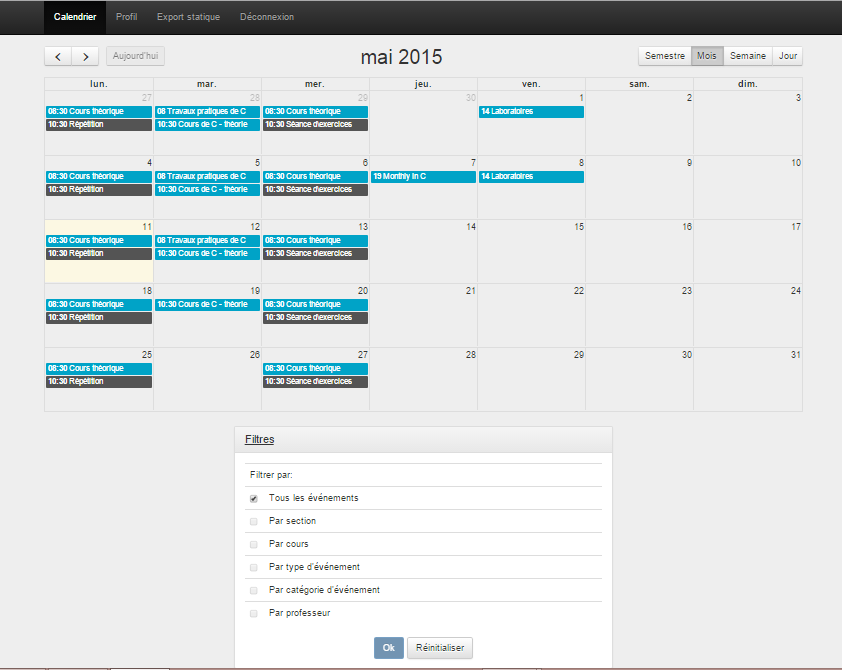
\includegraphics[scale=1.5]{calendar_page.png}}
	\subfigure{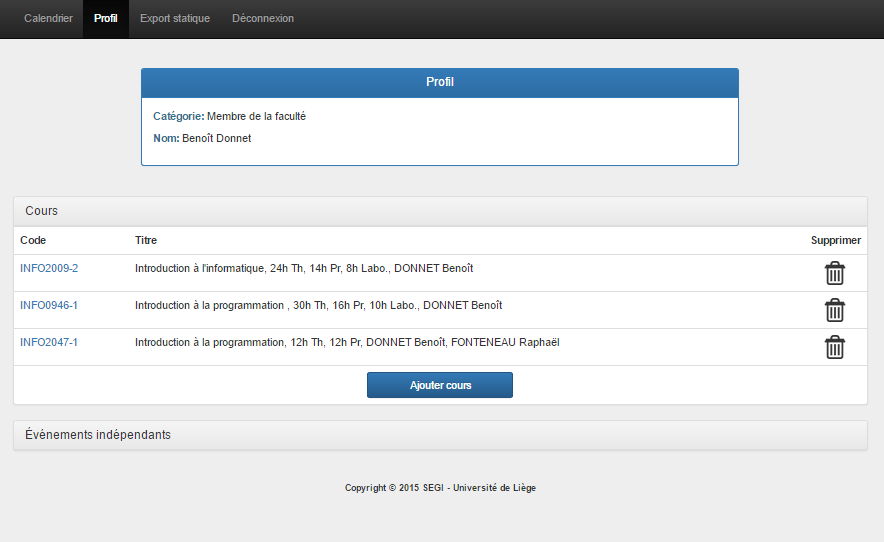
\includegraphics[scale=1.5]{profile_page.png}}
\end{figure}

\vfill{}

\begin{center}
    \textbf{Integrated Software Project (PROJ0010)}
\end{center}
\vspace{1cm}

\end{document}
